\chapter{Analysis}

\section{Average Time Calculated}
In the following data tables, the average time of the fall for each ball at 
each height is calculated

\begin{figure}[!h]
  \begin{minipage}{0.45\textwidth}
    \centering
    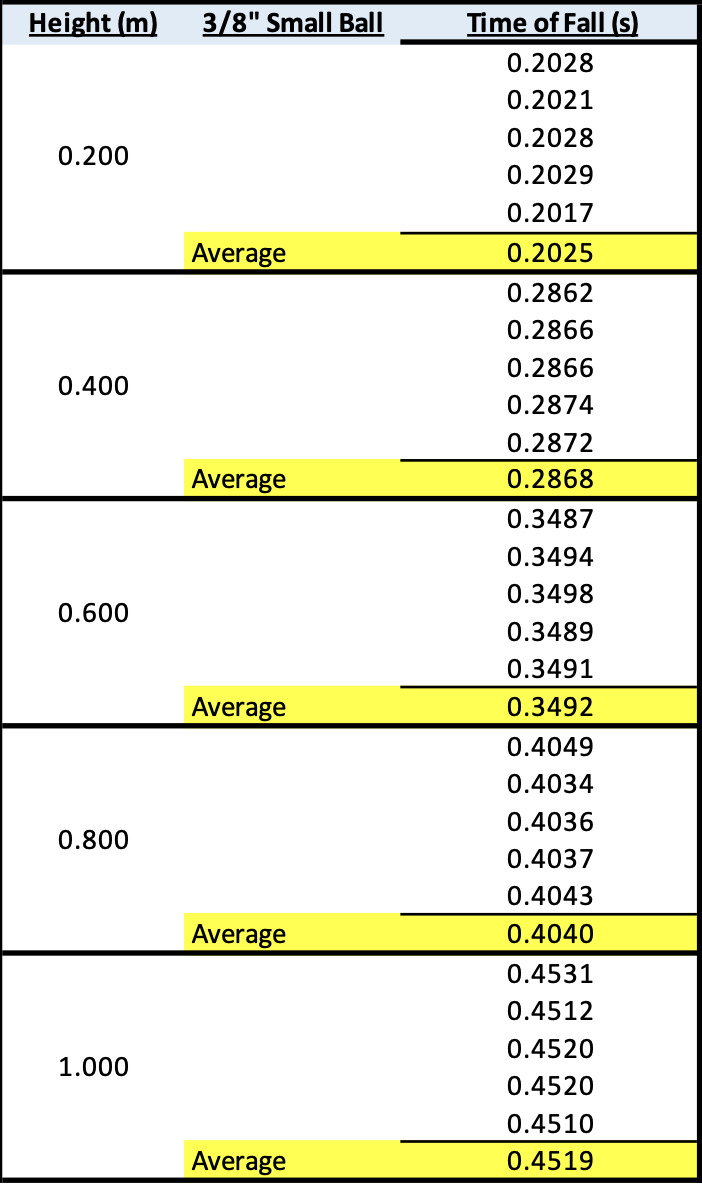
\includegraphics[scale=0.39]{resources/SmallTableAverage.jpg}
  \end{minipage}\hfill
  \begin{minipage}{0.45\textwidth}
    \centering
    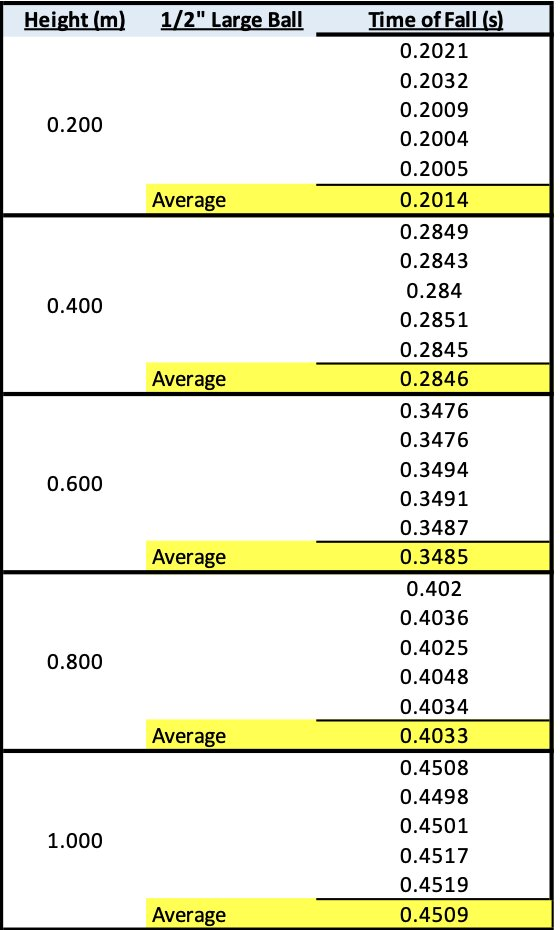
\includegraphics[scale=0.5]{resources/LargeAverageTable.jpg}
  \end{minipage}

\end{figure}


\newpage

\section{Graphed Data}
The following graphs for the small and large ball and their avaerge fall times
at each height squared then divided by 2, are plotted on a scatter plot and 
given a linear line with a calculated slope.


\begin{figure}[!h]
    \centering
    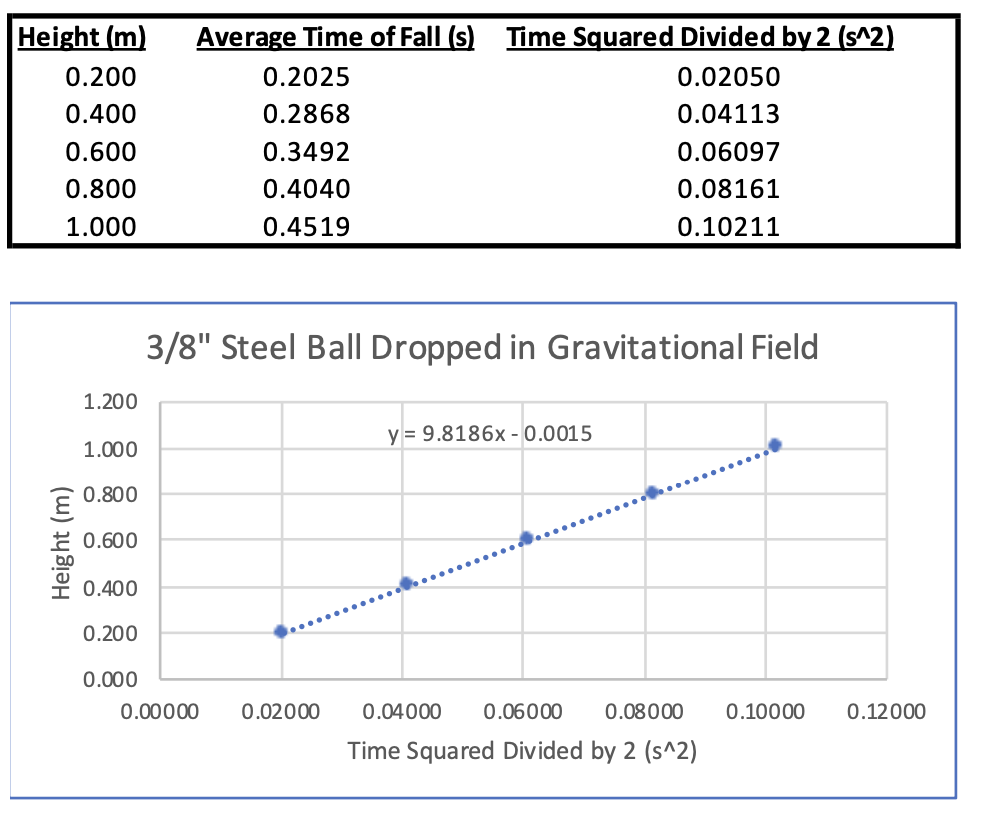
\includegraphics[scale=0.55]{resources/GraphSmall.png}
    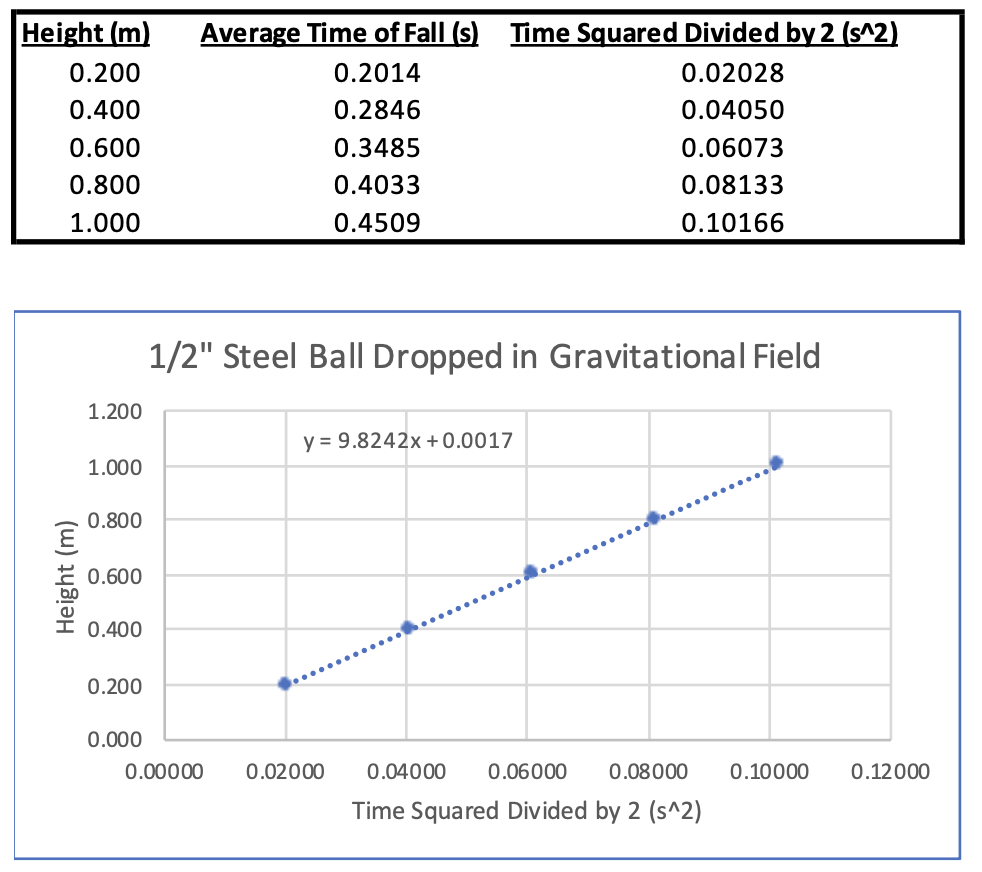
\includegraphics[scale=0.55]{resources/GraphLarge.png}
\end{figure}

\newpage

\section{Answers to Questions Posed by Lab}

\begin{enumerate}
  \item How is \underline{average} velocity different from \underline{average} speed? Tell the definition of each.\\
    ANSWER: Average speed only shows how fast an object is going which is the total distance over a total time.
    Average velocity shows both the direction and the magnitude of an object over a time.
  \item When, if at all, is the magnitude of the average velocity of an object moving in one-dimension:
  \begin{enumerate}
    \item equal to that object’s average speed? Explain\\
      ANSWER: The average velocity of an object moving in one-dimension is only equal to that object's
      average veolcity when dispalcement is equal to the distance i.e. an object is moving in one direction
    \item greater than that object’s average speed? Explain.\\
      ANSWER: The average velocity of an object moving in one-dimension is \textbf{never} greater than 
      that object's average speed. The displacement is always less than or equal to the direction.
    \item less than that objects average speed? Explain.\\
      ANSWER: The average velocity of an object moving in one-dimension is less than the average speed of
      that object when it changes direction. For example when an object moves then returns to wher it
      started.
  \end{enumerate}
\item In the absence of air resistance, should the values of $g_{exp}$ be the same or different for the two
    balls? Explain your answer.\\
    ANSWER: Due to the absence of air resistance and the equation $F=ma$, values of $g_{exp}$ for the two 
    different balls should be the same. This is because the gravitational force of acceleraton is not 
    dependent on mass.
\end{enumerate}
